\documentclass[12pt]{article}

\usepackage{amsmath}
\usepackage{graphicx,psfrag,epsf,amssymb}
\usepackage{enumerate}
\usepackage[top=1.0in, bottom=1.0in, left=1.0in, right=1.0in, headheight=1.0in]{geometry}
\usepackage{hyperref}
\usepackage{pdfpages} % To include activity worksheets
\usepackage{float}
\usepackage{natbib}
\usepackage{enumitem}
\newlist{todolist}{itemize}{2}
\setlist[todolist]{label=$\square$}

\newcommand{\blind}{0}

\newcommand{\todo}[1]{{\color{blue}[[\textbf{TODO: }#1]]}}

\date{December 15, 2019}

\begin{document}
\def\spacingset#1{\renewcommand{\baselinestretch}%
{#1}\small\normalsize} \spacingset{1}


%%%%%%%%%%%% DEFINING TITLE FOR PAPER & REMOVAL FOR BLIND VERSION %%%%%%%%%%%%%%

\if1\blind
{
  \title{\bf Designing Data Science Workshops for Data-Intensive Environmental 
  Science Research}
  \author{Allison Theobold \thanks{The authors gratefully acknowledge the 
  \textit{National Network of Library of Medicine}
    Data Engagement PNR grant for supporting this research.} \hspace{.2cm}\\
    Department of Mathematical Sciences, Montana State University \\
    Bozeman, MT \\
    allisontheobold@montana.edu \\
    and \\
    Stacey Hancock \\
    Department of Mathematical Sciences, Montana State University \\
    stacey.hancock@montana.edu \\
    and \\
    Sara Mannheimer \\
    Montana State University Library \\
    sara.mannheimer@montana.edu
    }
  \maketitle 
} \fi

\if0\blind
{
  \title{\bf Designing Data Science Workshops for Data-Intensive Environmental Science Research}
  \author{Anonymous}
  \date{}
  \maketitle
} \fi
%%%%%%%%%%%%%%%%%%%%%%%%%%%%%%%%%

\bigskip

\begin{abstract}
% currently 182 words 

Over the last 20 years, statistics preparation has become vital for a broad 
range of scientific fields, and statistics coursework has been readily 
incorporated into undergraduate and graduate programs. However, a gap remains 
between the computational skills taught in statistics service courses and those
required for the use of statistics in scientific research. Ten years after the 
publication of ``Computing in the Statistics Curriculum,'' the nature of 
statistics continues to change, and computing skills are more necessary than 
ever for modern scientific researchers. In this paper, we describe research on 
the design and implementation of a suite of data science workshops for 
environmental science graduate students, providing students with the skills 
necessary to retrieve, view, wrangle, visualize, and analyze their data using 
reproducible tools. These workshops help to bridge the gap between the computing
skills necessary for scientific research and the computing skills students 
leave their statistics service courses with. Open to faculty, staff, and the 
larger community, these workshops promote continued learning of the tools
necessary for working with data and provide additional resources for
incorporating data science into the classroom.

\end{abstract}

\noindent %
{\it Keywords:}  data science, data visualization, data wrangling, \texttt{R}, 
environmental science, workshops, reproducible research 

\vfill

\newpage
\spacingset{1.45}

\section{Introduction}
\label{sec:intro}

\quad Scientific fields have seen profound increases in the volume and variety 
of data available for analysis. Matched with the growth in computational power, 
today's scientific researchers are faced with computational and statistical 
expectations beyond those of the coursework dictated by their curriculum. In the
environmental sciences, though statistics courses have been readily incorporated
into undergraduate and graduate curricula, an abundance of literature suggests 
that these curricula fail to equip graduate students with the computing skills 
necessary for research in their field (Andelman et al., \citeyear{andelman}; 
Green et al., \citeyear{green}; Hampton et al., \citeyear{hampton}; Hernandez et
al., \citeyear{hernandez}, Mislan, Heer, \& White, \citeyear{mislan}; Teal et 
al., \citeyear{datacarpentry}; Theobold and Hancock, \citeyear{theobold}). Only 
one of these studies \citep{theobold}, however, acknowledges the substantial 
role statistics courses could potentially play in students' acquisition of 
computational skills. 

\quad Over the last 10 years, a large number of statistics educators have echoed
Nolan and Temple Lang's call to ``embrace computing and integrate it fully into 
statistics undergraduate major and graduate programs" (Nolan and Temple Lang, 
\citeyear{nolan}, p.\ 97; Baumer, \citeyear{baumer_datascience}; Baumer, Horton, 
\& Wickham, \citeyear{horton_takingachance}; Cetinkaya-Rundel and Rundel, 
\citeyear{mine}; Cobb, \citeyear{cobb}; Hardin et al., \citeyear{hardin}; Horton
and Hardin, \citeyear{horton_thinkwithdata}; Kaplan, \citeyear{kaplan}; McNamara
and Horton, \citeyear{mcnamara}). Indeed, the American Statistical Association 
Curriculum Guidelines for Undergraduate Programs in Statistical Science 
(\citeyear{asa}) reflect the increasing importance of data science skills.
Despite this campaign for computing in the statistics classroom, graduate-level 
statistics service courses have largely been overlooked, even though their 
potential impact is substantial. Unlike courses designed for an undergraduate or
graduate program in Statistics, these service courses often act as the sole 
exposure to computing with data prior to the start of a student's independent 
research. 

\quad The intention of this research is to (1) describe the computing skills 
necessary for research in the environmental sciences, (2) investigate how these 
skills can be infused into currently existing extracurricular workshops, and (3)
understand the experiences of attendees of these workshops. We investigated 
these areas of interest using a three-phase design-based implementation
research model \citep{penuel}. In the first phase, we conducted in-depth
interviews with faculty from environmental science fields regarding the
computational skills they believe are necessary for graduate students to succeed
in their research. Phase two then focused on adapting currently existing
workshop resources to design of a series of data science workshops targeting the
key computational skills distilled from these interviews. The final phase
consisted of implementing the workshops and collecting survey responses from the
workshop attendees regarding their experiences participating in each workshop.  

\begin{figure}[h!]
    \centering
    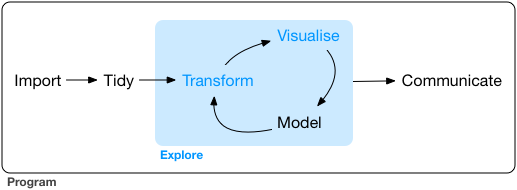
\includegraphics[width = \textwidth, height = 2in]{images/data-science-explore.png}
    \caption{Data Analysis Cycle, Wickham, H. \& Grolemund, G. (2017) \emph{R 
    for Data Science}. Sebastopol, California: O'Reilly.}
\label{fig:cycle}
\end{figure}

\quad For this research, the collection of disciplines who perform research 
across a variety of environmental science fields are captured under the term 
``environmental science.'' At our institution, these are the fields of Ecology, 
Land Resources nd Environmental Sciences, Plant Sciences and Plant Pathology,
and Animal and Range Sciences, whose students are required or highly recommended
to complete graduate-level statistics coursework for a masters or doctoral
degree. In this paper, the ``data analysis cycle'' consists of all stages in the
data analysis process, from data importation to data exploration to the
communication of results (Figure \ref{fig:cycle}), where data modeling is but
one component. The ``data science skills'' necessary to engage in this cycle may
include general programming concepts such as loops, user-defined functions, or 
conditional statements. However, the cornerstone of data science skills differs
fundamentally from general programming skills, with a focus on data rather than 
computer architecture, design, and applications. 

\quad We begin by outlining areas of research that address the computational and
statistical training of graduate students in the environmental sciences and the 
potential for extracurricular workshops to fill gaps in students' computational 
preparation. Next, we outline methodology used to design and implement a suite
of data science workshops tailored to environmental science graduate students. 
Section \ref{sec:faculty} summarizes the first phase of research, outlining the
computational skills faculty members identified as necessary for graduate
students to succeed in their independent research. Next, Section 
\ref{sec:workshops} discusses how these identified skills were interwoven into
existing data science workshop materials for researchers in the environmental
sciences. Section \ref{sec:implement} summarizes the backgrounds and experiences
of the workshop attendees during the 2018-2019 academic year, and describes the
research conducted on the implementation of the workshops. The resources used to 
facilitate the sustainability of these workshops is outlined in section 
\ref{sec:sustainability}, alongside possibilities for formally integrating these
workshops into the university curricula. Section \ref{sec:future} outline
future research plans for a second iteration of this design work. To close, we
revisit the current climate of computing in the statistics curriculum for
service courses and describe how these types of extracurricular workshops can
assist in further integration of computing into these classrooms. 

\section{The Current Climate of Statistics and Computing in the Environmental 
Sciences}
\label{sec:lit}

\quad Due to the substantial growth in the volume and variety of available data 
over the last two decades, the practice of environmental science has changed 
dramatically. Advances in technology have made computationally heavy 
applications of data science techniques---such as management and coalition of 
large data sets, high frequency spatial and temporal data visualization, and 
hierarchical Bayesian modeling---essential understandings for environmental 
science research. This flood of data has ``challenged the research community's 
capacity to readily learn and implement the concepts, techniques, and tools" 
\citep[p.\ 546]{hampton} necessary for data-intensive environmental science 
research, creating a crucial need to re-evaluate how our educational system can
better prepare current and future generations of researchers 
(\citeauthor{green}, \citeyear{green}; \citeauthor{hampton}, 
\citeyear{hampton}).  

\subsection{Computing in the Environmental Sciences Curriculum}

\quad Arising from a decade of mumblings about the importance of computing to 
research in the environmental sciences \citep{andelman, dodds1, dodds2, eglen, 
green, hastings, kelling, wilson-software-carpentry, wilson, wing}, 2010 brought
two studies on the computational ill-preparation of environmental students by
their curriculum. In the first large scale study of ecology instructors, 
Strasser and Hampton found that undergraduate students were not being prepared
with the data management tools necessary to engage in environmental science
research. Across 51 different institutions, despite largely affirming the
importance of data management skills, fewer than 20\% of instructors reported
data management topics in their courses. That same year, an environmental
science graduate student led a large scale study of the computational
experiences of future environmental scientists \citep[p.\ 1068]{hernandez}. In a
survey of environmental science graduate students across the United States, the
authors found that over 74\% of the students surveyed reported they had no
skills in any programming language---including \texttt{R}---and only 17\%
reported basic skill levels in any programming language. Hence, a large number
of students may be leaving their undergraduate and graduate programs without the
data science skills necessary for data-intensive research in their field. 
Hernandez and colleagues, however, noted that student-focused workshops could
work toward bridging this gap, by ``providing intensive environments'' where
students could learn ``particular methods or technologies'' (p.\ 1075).

\quad Due to the lack of ``training in data and computing skills'' 
\citep[p.\ 136]{datacarpentry} in undergraduate and graduate programs in the 
environmental sciences, external learning opportunities are necessary to prevent
researchers from continuing to teach themselves or each other everything they
know about data management and analysis. Out of these need for high-quality
resources for learning scientific computing emerged The Carpentries project
(\citeyear{carpentries}). The Carpentries focuses on teaching ``foundational
computational and data science skills to researchers'' through in-person,
hands-on, domain-specific workshops. As part of their educational mission,
The Carpentries collaboratively develops publicly available lessons for
populations of researchers, which do not assume that attendees have any prior
knowledge before attending the workshops. Teal and colleagues acknowledge that,
while these workshops ``will not be able to teach researchers all of the skills
they need in two days,'' workshops ``are a way to get started,'' lowering the
activation energy required to begin acquiring computing skills and empowering
researchers ``to be able to conduct the analyses necessary for their work in an
effective and reproducible way'' (p.\ 143). 

% The success of these workshops can be viewed as 
% a ``symptom of the current curriculum's shortcomings'' \citep[p.\ 547]{hampton}, 
% as there continues to exist a ``paucity of systematic training within university
% programs to equip students with the computational skills they need to conduct 
% data-intensive research'' (p.\ 547). 

\quad Over the last 20 years, statistical preparation in the environmental 
sciences has grown to be considered vital \citep{hampton}, and statistics
coursework has been integrated into graduate programs across the nation. Yet,
none of these conversations have acknowledged the substantial role students'
statistics education potentially plays in their attainment of the data science
skills necessary for research. Today, throughout their research, the majority of 
environmental science graduate students are required to produce code as part of
their data analysis process \citep{mislan}. To compound the difficulties these 
graduate students face, over this same period, the software used by
environmental science researchers has shifted, with an increase of over 45\%
in the use of \texttt{R} in environmental science publications since 2008
\citep{Rpopular}. The clear need for data science proficiency in environmental
science research necessitates a transformation of the environmental science
curriculum similar to that which infused statistics preparation into the
required graduate coursework. 

\subsection{Computing in the Statistics Curriculum}

\quad Changes in the digital age have also had ``a profound impact on statistics
and the nature of data analysis" \citep[p.\ 97]{nolan}, with today's skills 
differing substantially from what was needed but five to ten years ago. 
In the year following the publication of ``Computing in the Statistics 
Curriculum'' \citep{nolan}, the Mckinsey Report \citep{mckinsey} was published. 
The McKinsey report stated that, by 2018, ``the United States alone could face a
shortage of 140,000 to 190,000 people with deep analytical skills as well as 1.5
million managers and analysts with the know-how to use the analysis of big data
to make effective decisions'' (p.\ 3). With calls to transform the undergraduate
statistics curriculum resounding nationally, the 2014 American Statistical 
Association (ASA) President, Nathaniel Schenker, convened a workgroup to update
the association's guidelines for undergraduate programs. These new guidelines 
included an increased emphasis on data science skills and real applications, 
specifically students' ability to ``access and manipulate data in various ways,
use a variety of computational approaches to extract meaning from data, program
in higher-level languages" \citep[p.\ 7]{asa}. 

\quad With this curricular momentum, in 2015, \emph{The American Statistician} 
produced a special issue on ``Statistics and the Undergraduate Curriculum,'' to
encourage submissions of broader topics in the statistics curriculum. Articles 
in the special issue ranged from detailing how computing should be included 
throughout the Statistics curriculum \citep{jenny, tintle, hesterberg}, to 
presenting thoughts on how data science topics should be integrated into 
undergraduate statistics courses, \citep{esr, grimshaw, 
baumer_datascience, hardin}. In the same issue, George Cobb provocatively stated
that the statistics curriculum needed to be rebuilt ``from the ground up'' 
(\citeyear{cobb}), as ``what we teach lags decades behind what we practice'' and
``the gap between our half-century-old curriculum and our contemporary 
statistical practice continues to widen'' (p.\ 268). Moreover, despite the 
issue's focus on the broader statistics curriculum, statistics educators
continued to lament that the current Introductory Statistics curriculum teaches
a snapshot of the entire data analysis cycle, ``wherein challenges with data
computational methods, and visualization and presentation are typically elided'' 
\citep[p.\ 336]{baumer_datascience}. 

\quad The following year, however, brought the revised GAISE college report 
\citep{gaise}, creating a push for reform in the Introductory Statistics 
curriculum. The six recommendations originally outlined by the committee in 2005
continued, but the authors suggested two new emphases for the first
recommendation (teach statistical thinking), which better reflect the modern
practice of statistics. First, statistics educators should ``teach statistics as
an investigative process of problem-solving and decision making,'' and should 
``give students experience with multivariable thinking'' (\citeyear{gaise}, 
p.\ 3). These recommendations reiterate the sentiments heard throughout the
statistics community, that students should emerge from our courses with the
understanding that data analysis ``isn't just inference and modeling, it's also
data importing, cleaning, preparation, exploration, and visualization'' 
\citep{mine-jsm}. Yet, the inclusion of these topics in the Introductory 
Statistics curriculum is still a heated discussion. Many educators continue to 
believe (1) that it is not possible to teach statistical concepts and 
programming in just one course, (2) that teaching programming takes up valuable
time which could be used towards teaching important statistical concepts, or 
(3) students are not interested in learning to program \citep{mine-jsm}. Thus, 
despite charges for the statistics community to ``treat computing as fundamental
as basic mathematics and writing'' \citep[p.\ 298]{esr}, many students leave
their Introductory Statistics course without ``a set of practices and attitudes
about data that are immediately applicable to their lives'' 
\citep[p.\ 309]{gould}. 

\quad Amidst these conversations, \texttt{R} packages were being created, which 
would fundamentally changing how users interact with \texttt{R}. These 
\texttt{R} packages, universally known as the ``\texttt{tidyverse},'' have 
created user friendly \texttt{R} tools which ``share an underlying design 
philosophy, grammar, and data structures'' \citep{tidyverse}. Statistics 
educators have begun to leverage these tools in the Introductory Statistics 
classroom to teach reproducibility \citep{mine-rmarkdown}, data management 
\citep{horton_takingachance}, dynamic data \citep{hardin-tise}, and big data
\citep{horton-tise}. While there exists a growing momentum to incorporate these
new \texttt{R} tools into the Introductory Statistics classroom, attention has 
yet to be paid to alternative statistics service courses, such as those taken 
by environmental science graduate students. These courses, like Introductory 
Statistics, serve graduate students from a variety of scientific backgrounds. 
However, unlike an undergraduate Introductory Statistics course, students are 
expected to emerge from their statistics coursework with the statistical and 
data science skills necessary for their research. 

\quad The frustrations echoed by environmental science educators 
\citep{hampton, datacarpentry} suggest that, despite the inclusion of statistics 
coursework into these graduate programs, students continue to leave the 
statistics classroom without the data science skills necessary to participate in 
the data analysis cycle in their own research. The fundamental question raised 
ten years ago by Nolan and Temple Lang still applies today: do our students
leave the statistics classroom able to ``compute confidently, reliably, and
efficiently?'' (\citeyear{nolan}, p.\ 100). An in-depth study of environmental 
science graduate students' experiences acquiring the computing knowledge
necessary for their research answered this question with a resounding `no' 
\citep{theobold}. Like the hypothesis of Teal and colleagues (2015), these
students did not attribute their acquisition of the data science skills
necessary for their research to the statistics courses they took for their
degree. Rather, students gained the data science skills necessary to engage in
the entire data analysis cycle through independent research experiences, an
``all-knowing'' past or current graduate students, and peer networks. Ten years 
after the publication of ``Computing in the Statistics Curriculum,'' we continue
to assume that ``students will `pick up' the skills they need'' to participate 
in the data analysis cycle outside of their statistics coursework 
\citep[p.\ 309]{gould}. 

\subsection{Extracurricular Workshops to Bridge the Gap}

\quad Reiterated by both statistics education and environmental science 
researchers alike \citep{nolan, datacarpentry}, this lack of training in 
computational skills impedes the progress of scientific research, sends the 
signal to students that computing is not of intellectual importance, and is 
laden with hidden costs. Students may pick up bad habits, misunderstandings, or 
the wrong concepts, learn just enough to get what they need done, spend weeks or
months on tasks that could be done in hours or days, and they may be unaware of 
the reliability and reproducibility---or lack there of---of their results (Nolan
and Temple Lang, 2010, p.\ 100; Teal et al., 2015, p.\ 136). But why are these
skills still so rarely included in these service courses when the need for them
is widely recognized?

\quad Environmental science educators have reiterated the challenges in 
integrating computing into the curriculum outlined by Nolan and Temple Lang. 
These barriers can be boiled down to ``attempting to fit more material into
already-full courses and curriculum, which are taught by people who do not feel
prepared to address topics relevant to big data and data-intensive research'' 
\citep[p.\ 547]{hampton}. These hurdles are potentially even greater for 
graduate-level statistics service courses. Instructors of these courses are 
often explicitly told the statistical content students are expected to learn, 
while it is implicitly assumed they are also teaching students the data science
skills necessary for them to participate in the entire data analysis cycle.
Claiming these graduate students ought to take additional, data science specific
courses to obtain these skills is infeasible for many, as graduate programs
frequently leave little room for additional coursework. 

\quad Until computing has been meaningfully integrated into these service 
courses, extracurricular workshops hold the potential to address the gap between
the computational preparation of students by their coursework and the 
computational requirements of their research. Although data science skills can 
potentially be acquired from the drove of currently available online resources, 
such as online lessons, MOOCs and books, none of these resources provide
researchers with the ability to pose their questions directly to an instructor
or to learn from others. Moreover, this drove of online materials, poses a  
``significant challenge in being able to discover relevant and high-quality
materials,'' for researchers with limited time. 

\quad As, reiterated by Nolan and Temple Lang (\citeyear{esr}), extracurricular
learning opportunities are not a direct substitute for the prolonged instruction
of these skills that occurs in a course. However, this is not the goal 
of these learning opportunities. Instead, short, intensive workshops, such as
those provided by The Carpentries, are able to teach immediately useful skills
that can be taught and learned quickly, keep learners active by using live
coding and formative assessment, work with a learners from a variety of
backgrounds, and build learners' self efficacy \citep{null-carpentries}, so that
attendees ``learn the computational aspects as part of an interesting, 
challenging, and confidence-building process'' \citep[p.\ 101]{nolan}.

\section{Methodology}

\quad Improving environmental science graduate students' access to ``powerful,
effective learning opportunities'' \citep[p.\ 137]{penuel} necessitates
understanding the skills required for these students to be successful in their
research. Design-based implementation research (DBIR) \citep{confrey, penuel,
oneill} ``offers a model for the design and testing of innovations
within the crucible of classrooms and other contexts for learning'' 
\citep[p.\ 140]{penuel}. Rather than creating workshops covering content outside
parties believe are important, DBIR uses collaboration with members of the
community to develop ``evidence-based improvements'' (p.\ 143) to teaching 
innovations---situating community members as ``co-designers of solutions to 
problems'' \citep[p.\ 140]{penuel} rather than bystanders. 

\quad This paper describes the results of the first iteration of this DBIR, 
consisting of three phases. Section \ref{sec:faculty} summarizes phase one which 
investigated the computing skills necessary for graduate-level environmental
science research. Phase two of this research, described in Section 
\ref{sec:workshops}, details how the skills identified during phase one were
used to tailor currently existing Data Carpentry \citeyear{data-carpentry} and
Software Carpentry \citeyear{software-carpentry} lessons to meet the needs of
environmental science graduate students. Finally, Section \ref{sec:implement}
chronicles the third phase of this research, implementing and evaluating these
workshops. This final evaluation phase focuses on the survey results of the 
backgrounds and experiences of workshop attendees, rather than the workshop
content or learning outcomes of attendees, which are described as directions for
future research. 


\section{Outlining the Computing Skills Necessary for Environmental Science
Research}
\label{sec:faculty}

\quad As the direct supervisors of graduate students, environmental science
faculty members are potentially aware of the computing skills that are vital to
researchers in their respective fields. Thus, interviews with faculty members
from these fields allow for us to gain an understanding of the essential skills
required of environmental science graduate students. 

\quad In the spring of 2017 and fall of 2018, every faculty member in the
Ecology, Land Resources and Environmental Sciences, Animal and Range Sciences, 
and Plant Sciences and Plant Pathology departments, currently overseeing a
graduate student were emailed requesting their participation in this research. 
While some faculty enthusiastically agreed to participate, others declined for
three main reasons---they hadn't directly overseen a graduate student recently,
they deemed themselves to be weak in statistics, or they were unavailable to
meet. Table \ref{tab:faculty} outlines the number of faculty requested for
participation and the number of faculty interviewed, by departmental
affiliation. 

{\spacingset{1.05}
\begin{table}[h!]
\centering
\begin{tabular}{lcc}
\hline
Department & Faculty Invited & Faculty Interviewed  \\
\hline
Animal \& Range Sciences & 7 & 2 \\
Ecology & 15 & 8 \\
Land Resources and Environmental Sciences & 24 & 8 \\
Plant Sciences \& Plant Pathology &  15 & 5 \\ 
\hline
\end{tabular}
\caption{Number of faculty members requested for participation and interviewed,
by department.}
\label{tab:faculty}
\end{table}
}

\subsection{Data Collection}  

\quad The faculty members who agreed to participate, engaged in a one-hour 
interview regarding (1) the computational skills they believe are necessary for
masters and doctoral students to implement statistics for research in their
field, and (2) how they believe graduate students acquire these necessary
skills. The full interview protocol as supplementary material 
\footnote{Materials associated with this manuscript are available at 
\href{https://github.com/atheobold/data-science-workshops-jse}{https://github.com/atheobold/data-science-workshops-jse}}.  

% \quad Based on faculty's responses, the interviewer asked follow-up questions to
% further explore why the faculty believe the computational skill(s) in question 
% are necessary. For instance, if a faculty voiced the need for students to be 
% able to build a data workflow, further information was sought regarding what 
% specific computing skills this would require. Alternatively, when the response 
% from faculty consisted of the statistical understandings necessary for graduate
% student researchers, follow-up questions were asked to delve further into what
% computing skills a student may require to successfully implement this type of
% statistical analysis with their data. Not only did these interviews provide
% valuable feedback on \emph{what} content the workshops should include, they also
% added insight into \emph{why} workshops form an ideal mode of delivery for this
% needed training.  

\subsection{Data Analysis} 

\quad The primary author led a three-stage data analysis process (Miles, 
Huberman, Salada$\tilde{\text{n}}$a, \citeyear{miles}). During the first stage,
the interviews for every faculty member were transcribed verbatim. Following 
this process, the primary author read the transcripts independently, 
highlighting excerpts where computing skills were discussed. The author then 
created descriptive codes for the skills faculty identified as necessary in each
of these excerpts. At the close of this stage, the author examined these codes 
for specific references to computing skills currently addressed in Data 
Carpentry's \emph{Data Analysis and Visualization in \texttt{R} for Ecologists} 
lesson \citep{ecology_curriculum}. 

% Why only look at this curriculum? 

\quad Following this process, the primary author began the second stage of 
analytical coding, synthesizing descriptive summaries into instances of a
general concept \citep[p.\ 95]{miles}. During this stage, skills were linked
thematically, and themes that held across multiple interviews were retained.
Next, the author searched through these themes to uncover how each theme related
to the others. Through this process it was determined that certain themes 
captured similar constructs, and were merged into a single theme, whereas other
constructs were voiced independently, and separate themes were formed. For
example, while every faculty voiced students' need to work with data in 
\texttt{R}, these sentiments were voiced alongside students' need to perform
other data wrangling operations, such as reorganize data, filtering out rows of
data, selecting columns, creating new variables, or modifying existing
variables. Hence, the themes of ``working with data'' and ``data wrangling''
were merged into the single theme of ``working with data.'' Alternatively, while
reproducibility is a key aspect to working with data in \texttt{R}, faculty
sentiments regarding the need for students' work to be reproducible was not
voiced alongside a specific software.

\quad In the final stage of the analysis, the primary author searched the 
faculty transcripts for evidence supporting the emerging themes, scrutinizing 
whether each identified skill fit into the identified themes. Following this 
validation process, the first and second authors met to discuss the rationale
for each code and inspect the skills identified by faculty in the context of the
emergent themes. These final themes provide evidence for designing data 
science workshops for environmental science graduate students. 

\subsection{Skills Identified by Environmental Science Faculty}

\quad While some faculty had difficulties disentangling the statistical methods
students use in research from the computing required to implement those methods,
many were able to express the computing skills necessary for graduate students
in their field to engage in the entire data analysis process. A substantial
overlap was seen between faculty expectations and the ``data acumen'' outlined
by NAS \citep{nas}, falling into three categories: (1) working with and
wrangling data, (2) data visualization, and (3) reproducibilty.

\subsubsection{Working with Data}  

\quad Every faculty member interviewed believed that students' experiences in the
statistics classroom do not adequately prepare students to work with and
organize large, messy datasets. As graduate students perform their research,
they are required to think about ``storing data, managing data, matching
data, and collating data,'' into a meaningful datasets for analysis. Some 
faculty, aware of the different types of data their students work with, 
reflected that it is ``not uncommon to be analyzing half a million records, but
I think it's uncommon to be doing it effectively or efficiently.'' 

\quad These skills for working with data ranged from students' ability to 
``organize their data and get it in a way that can be used by \texttt{R}'' to 
tasks that required reorganizing data formats from wide to long or vice 
versa---a skill which every faculty member griped is not acquired through the
standard curriculum. A faculty member bemoaned that standard examples in
statistics courses provide students with data which are the product
of cross-tabulation, so students are never forced ``to figure out how to get the
cross-tabulation [they] need, so that [they] can bring it into \texttt{R} and do
[their] regression.'' These concerns reiterate the importance of ``data
management and curation'' detailed by NAS, who stated that ``at the heart of
data science is the storage, preparation, and accessing of data'' 
\citep[p.\ 26]{nas}. 

\subsubsection{Data Visualization} 

\quad The importance data visualization plays in every stage of students'
research was emphasized by every faculty member interviewed. Faculty affirmed
that students should possess the ability to create visualizations of their data
early and often. These expectations align with the the facility outlined by NAS
(\citeyear{nas}), who stated that students need to have the ability to ``present
data in a clear and compelling fashion'' (p.\ 26). One faculty member declared
that students' ability to look at their data in different ways dramatically
shapes their research potential, and the tools available today allow for
researchers to create visualizations precisely tailored for each investigation.
Many faculty voiced the usefulness of the \texttt{ggplot2} package \citep{ggplot} 
lowering the barriers for students to learn ``how to visualize [their] data to
explore and understand it.'' 

\subsubsection{Reproducibility}  

\quad Every faculty member emphasized the usefulness of ``manipulating data in
ways that are repeatable,'' through scripted programs such as \texttt{R}. Across
environmental science disciplines, faculty concurred that many students do not
use \texttt{R} for data wrangling, and instead rely on Excel because ``the code
(\texttt{R}) is kind of a black box'' and when they ``don't have that instant
connection with [their] data, I think it fundamentally boils down to fear.'' 
Concerns were raised for the students using unreproducible tools to wrangle
their data, as ``they would never find [their] way back to what the original
data set would have been'' and their advisers would have no way to understand
why certain data are missing. While many advisers stated that they encourage
students to avoid these brute force Excel manipulations, they reflected that 
students may not have the computing skills necessary to perform the same data
wrangling task in a scripted and reproducible manner. These faculty concerns
parallel the ``workflow and reproducibility'' acumen outlined by NAS, who stated
that students need to ``be exposed to the concept of workflows'' 
\citep[p.\ 28]{nas}. 

\subsubsection{How Students Gain Computational Skills}

\quad Across environmental science disciplines, faculty stated that they 
assume students are acquiring the computing skills necessary to analyze their 
data either in their required statistics coursework or on their own. When asked
why students are not acquiring computing skills in their field-specific courses,
a faculty member stated, ``We don't really have anyone to teach that. It's not
that it isn't valuable, but there is no one to teach it.'' Some faculty believed
``most graduate students come in knowing more about the tools one might use to
manipulate data than their advisers do,'' while others lamented the gaps between
the computational skills of their graduate students and their own training,
feeling ``personally out of touch [with students] because I haven't taken the
time to learn \texttt{R}, because of my training and my age.''These gaps impact
the assistance faculty can provide to their students, as ``increasingly faculty
feel that they're not at the forefront of their programming abilities, so their
students are being self-taught and are often computationally ahead of them.''

% \quad Although faculty feel that there may exist gaps between their own
% knowledge of working in \texttt{R} and their students', every faculty member
% affirmed the importance of students acquiring the computational abilities needed
% to perform data-intensive research. Indeed, it is not necessary for every
% student to be an expert, but faculty underscored the value of resources for
% students to acquire these computational skills necessary for their research. The
% majority of faculty voiced that it is often assumed that graduate students
% should be able to analyze their data because they've taken a statistics course.
% Yet, faculty members acknowledge the poor computational preparation of their
% students---even after taking a statistics course---and thus ``encourage
% [students] to use anything they can find to get more tools in [their] tool
% box.'' 

\section{Designing Data Science Workshops for Graduate Students in the 
Environmental Sciences}
\label{sec:workshops}

\quad The second phase of this research attended to the  development of a suite
of data science workshops targeted to graduate students in the environmental
sciences. Skills identified through faculty interviews were incorporated into a
set of four 3-hour workshops covering (1) the basics of programming in 
\texttt{R}, (2) intermediate programming tasks in \texttt{R}, (3) creating
appropriate and effective data visualizations, and (4) cleaning and merging data
in preparation for analysis and visualization, all using reproducible tools. 

\quad The materials for these workshops were adapted from Data Carpentry's 
\emph{Data Analysis and Visualization in \texttt{R} for Ecologists} lesson 
\citep{ecology_curriculum}, a curriculum maintained by experienced researchers
in ecological fields, which uses ecology-specific data contexts \footnote{This
work is a derivative of \emph{Data Analysis and Visualization in \texttt{R} for
Ecologists} \href{https://datacarpentry.org/R-ecology-lesson/}{(https://datacarpentry.org/R-ecology-lesson/)}
by Data Carpentry, used under CC-BY 
\href{https://creativecommons.org/licenses/by/4.0/}{(https://creativecommons.org/licenses/by/4.0/)}.}.
Importantly, the first workshop in \emph{Data Analysis and Visualization in 
\texttt{R} for Ecologists} does not assume that attendees have any previous
experience working in \texttt{R}, and each workshop builds on knowledge acquired
at previous workshop(s), without the expectation that attendees have acquired
additional knowledge or skills between workshops. The workshop materials
developed for this research are available through GitHub
\footnote{\href{https://github.com/atheobold/data-science-workshops-jse}{GitHub
repository (link)}}, with video tutorials recorded and available through our
institution's library 
\footnote{\href{http://bit.ly/ws_recordings}{MSU Library videos (link)}}.  

%  Data Carpentry materials are freely available under the \href{https://creativecommons.org/licenses/by/2.0/}{Creative Commons Attribution License}, for re-use or adaptation

\subsection{Data Context}  

\quad Emphasized by both the NAS and these faculty, ``effective application of
data science to a domain requires knowledge of that domain'' \citep[p.\ 29]{nas}. 
Hence, data science instruction ought to be grounded in ``substantive contextual
examples,'' to ``ensure that data scientists develop the capacity to pose and
answer questions'' with data relevant to them (\citeyear{nas}, p.\ 30). 
Therefore, ecological data are used for these workshops, originating from 
Montana Fish, Wildlife, and Parks and the Portal Project Teaching Database 
\citep{portal_data}. These data highlight a variety of aspects that
commonly occur in ecological data, including multiple sampling instances,
mark-recapture, biological measurements, and meta- and micro-level data. 

\subsection{Computing Tools for Environmental Science Research}  

\quad The structure and context of these workshops include a statistical
programming language used extensively throughout environmental science research
(\texttt{R}), environments which facilitate the learning of \texttt{R}
(RStudio and RStudio Cloud), and tools that promote reproducibility throughout
the entire data analysis cycle (R Markdown).

\subsubsection{Why \texttt{R}?} 

\quad The use of \texttt{R} is widespread throughout the environmental science
research community, a dramatic change over the last decade \citep{Rpopular}. 
Furthermore, with the invention of the RStudio IDE \citep{rstudio}, this
user-ship continues to increase, as \texttt{R} includes over 100 packages
frequently used in ecological data analysis \href{https://CRAN.R-project.org/view=Environmetrics}{(https://CRAN.R-project.org/view=Environmetrics)}. \texttt{R} is free and open source, so
attendees learn a statistical programming language that will be accessible to
them throughout their careers. Unlike MARK, VORTEX, or RMAS, with \texttt{R}, 
attendees results do not depend on remembering the sequence of buttons they
clicked. With the shocking realization that large numbers of modern scientific
findings cannot be replicated \citep{economist, johnson} and the growing
appreciation for reproducible data analysis methods in ecological research
\citep{reproducibilty-comment, repeatability, pva, reproducibility_ecology},
today's researchers in scientific fields are becoming more aware of the need for
a reproducible data analysis workflow. 

\subsubsection{Why RStudio?}

\quad RStudio is a free computer application that allows you access to the 
resources of \texttt{R}, while providing you with a comfortable working
environment \citep{rstudio}. The RStudio IDE ``makes [programming] less
intimidating than the bare \texttt{R} shell" \citep[p.\ 59]{mine}. Additionally,
the RStudio environment is consistent across operating systems, which is not the
case for other statistical software packages. Moreover, because RStudio is an
IDE, it includes integrated help files, intelligent code completion, and syntax 
highlighting---all of which help to reduce the learning curve. 

\subsubsection{Why RStudio Cloud?} 

\quad The RStudio Cloud was created as a platform to make it easy to do, share,
teach, and learn data science using \texttt{R} \citep{RStudioCloud}. Through the 
Cloud, attendees are able to access publicly available workshop materials, 
without worrying about software installation, package installation, or
transferring data. Workshop participants interact with the workshop's materials
in the same manner as a locally installed version of RStudio, as seen in Figure
\ref{fig:cloud}, and an organized RStudio project directory exposes attendees to 
best practices for reproducible project construction. 

\begin{figure}[t!]
    \centering
    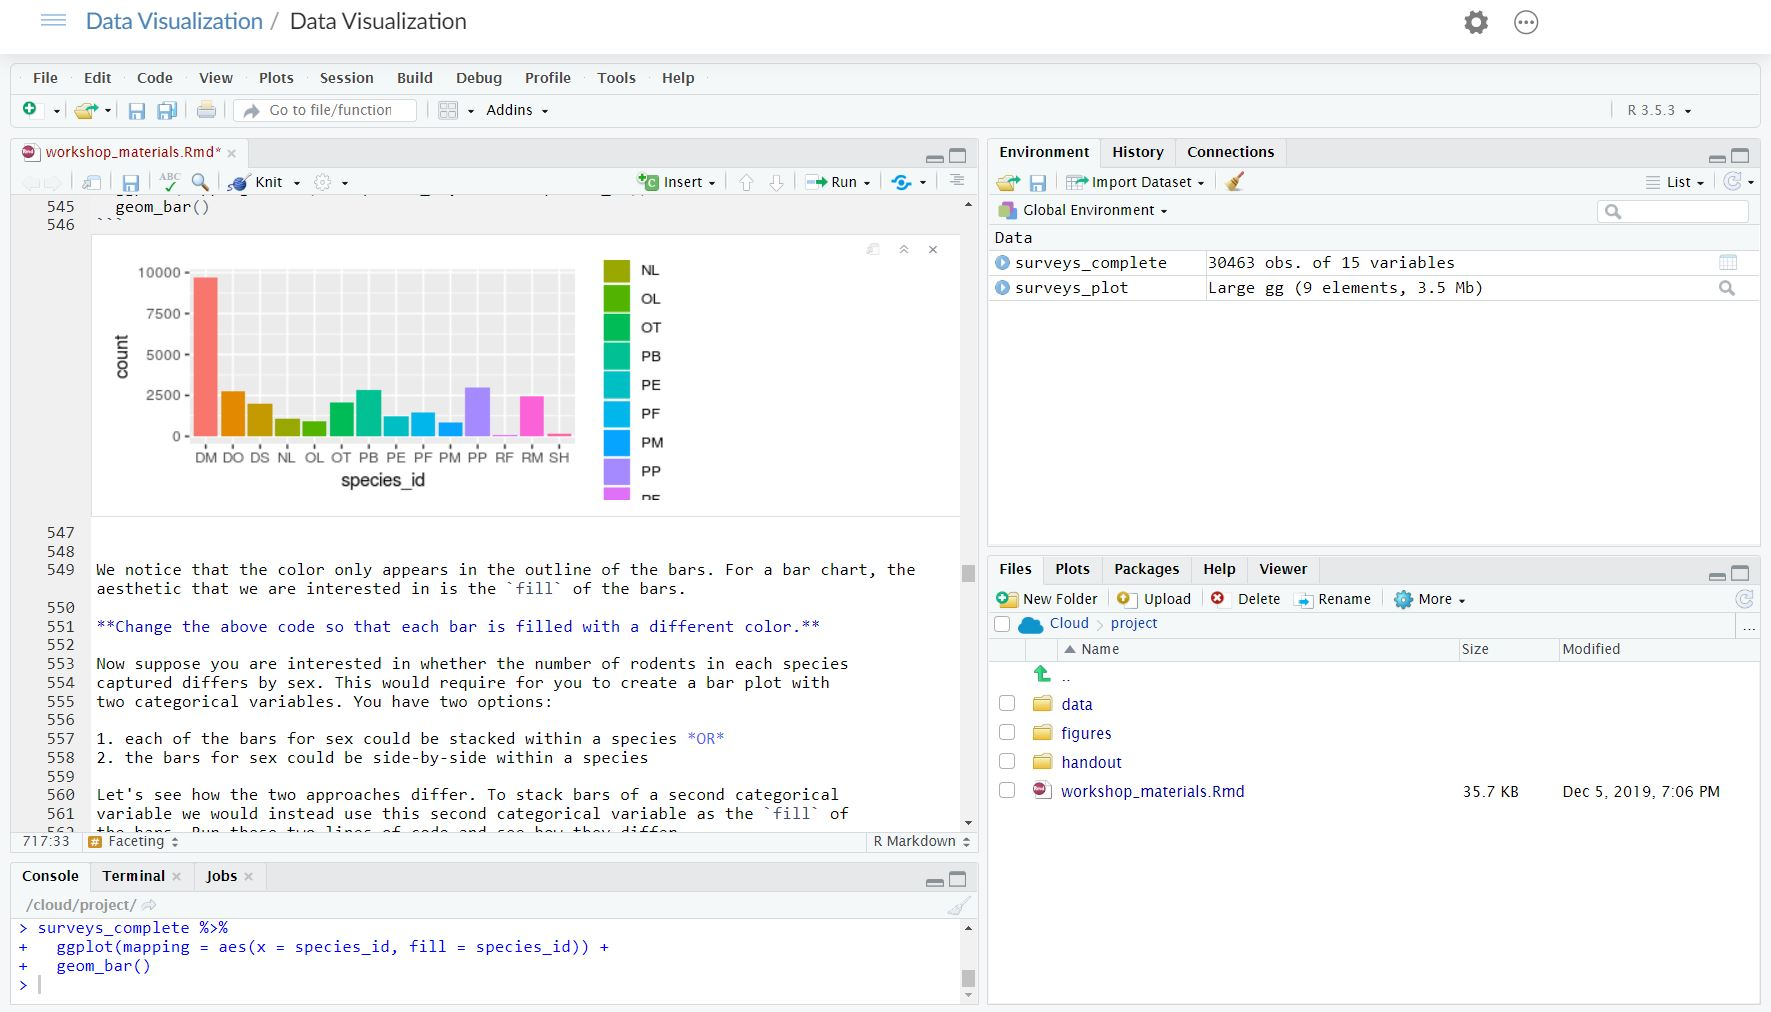
\includegraphics[width = \textwidth]{images/RStudio_Cloud_blind.png}
    \caption{RStudio Cloud workspace environment for \emph{Data Visualization
    with \texttt{ggplot2}} workshop. Every workshop works in an RStudio project,
    containing a master R Markdown file, a data folder containing the
    data used in the workshop, and the handout produced for attendees.} 
    \label{fig:cloud}
\end{figure}

\subsubsection{Why R Markdown Documents?}

\quad R Markdown documents provide an easy-to-understand framework to combine
statistical computing and written analysis in a single document, helping to
break the copy-paste paradigm for generating statistical reports 
\citep{mine-rmarkdown}. During the workshop, R Markdown documents allow for 
attendees to keep their code organized and their workspace clean, which is
unnatural for new learners. Each workshop's master R Markdown document contains
blocks of code and descriptions for every topic covered, allowing for
participants' exploratory work to be saved within a topic. For additional
information on R Markdown documents see \citeauthor{mine-rmarkdown} 
(\citeyear{mine-rmarkdown}). 

\subsection{Workshop Content}

\subsubsection{Introduction to \texttt{R}}
\label{sec:introR}

\quad This first workshop in the series covers the basics of learning to program
in \texttt{R}. The workshop first introduces the RStudio environment and project
work flow in RStudio, discussing project working directories and relative paths.
Next, the workshop progresses through tools for working with vectors and lists 
of different data types, motivating methods for working with dataframes. After
learning how to import data into \texttt{R}, the workshop proceeds through
inspecting data, extracting data, and changing data types. Motivated by working
with missing data, the workshop introduces \texttt{R} help files to inspect
function arguments and their default values. These help files are called upon
as participants make use of base \texttt{R} functions to create data summaries,
perform simple data cleaning, and produce both univariate and bivariate
visualizations of the data. 

\subsubsection{Intermediate \texttt{R}}
\label{sec:intermed}

\quad This second workshop covers coding skills to modularize \texttt{R} code. 
The content in this workshop, excluding relational statements, is not
included in Data Carpentry's \emph{Data Analysis and Visualization in \texttt{R}
for Ecologists} lesson. Instead, many of these concepts are covered in Software
Carpentry's \emph{\texttt{R} for Reproducible Scientific Analysis} lesson. Yet,
conditional statements, for-loops, and user-defined functions are skills that
many environmental science faculty asserted were necessary for graduate students
to possess as they perform independent research. 

\quad First, the workshop then progresses through the use of relational
statements and how to link these statements using and (\texttt{\&}), or
(\texttt{|}), and not (\texttt{!}) conjunctions. Next, the workshop dives into
the use of conditional statements, stepping from \texttt{if}, to \texttt{if
else}, to \texttt{else if} statements. The second half of the workshop covers
methods to iterate or replicate a set of instructions many times. Looping,
specifically \texttt{for()} loops, are introduced as a popular way to iterate or
replicate the same set of instructions. Working through exercises which
repeat operations on a dataset using both a \texttt{for()} loop and a recursive 
\texttt{for()} loop, motivate a discussion of why \texttt{R} users recommend the
use of vectorization for non-recursive \texttt{for()} loops. To conclude,
functions are presented as an approach to replicate the same set of instructions
in multiple locations throughout your code. Motivated by a script which copies 
and pastes the same process multiple times, attendees understand why this is 
an undesirable practice. Attendees are then tasked with transforming the
copy-paste-modify process into a function. By parsing out the function writing
process into a set of steps that should be used when you have copied and pasted
your code multiple times, participants leave with a foundational understanding
of why functions are useful and practical approaches for implementing them in
their own code.

\subsubsection{Data Wrangling with \texttt{dplyr} and \texttt{tidyr}}
\label{sec:wrangle}

\quad The \emph{Data Wrangling} workshop introduces common data wrangling issues
faced by environmental science researchers. Inspired by the difficulty of
reading bracket subsetting and how cumbersome it can be to remember the
different base \texttt{R} functions and formats to wrangle your data, this
workshop introduces the \texttt{dplyr} \citep{dplyr} and \texttt{tidyr} 
\citep{tidyr} packages. Much of \texttt{R}'s language has not changed over the
last 20 years, which leaves the desire for a ``smoother, more efficient, and
more readable pipeline for modern \texttt{R} workflows'' (Ross, Wickham, 
\& Robinson, \citeyear{tidytools}, p.\ 19). The \texttt{tidyverse} packages
share common interfaces and data structures that make it simpler to learn data
wrangling tasks and allow for the process to flow naturally from one step to the
next. 

% Add references to how the tidyverse simplifies cognitive load when learning to program in R

\quad The workshop begins by outlining six of the common ``verbs'' that handle
common data wrangling challenges, included in the  \texttt{dplyr} package: 
\texttt{select()}, \texttt{filter()}, \texttt{mutate()}, \texttt{group\_by()},
\texttt{summarise()}, and \texttt{arrange()}. Prompted by the need to perform a
sequence of multiple data wrangling operations, participants learn how to
connect each of these data wrangling verbs using the pipe operator 
(\texttt{\%>\%}). Next, motivated by the need to integrate additional data files
for analysis, the concept of relational data is outlined. After an introduction 
to key-value pairs, attendees make use of the \texttt{left\_join()} and 
\texttt{right\_join()} functions to join these additional data files. 

\quad The final topic of the workshop involves the issue of data reorganization.
Until now, participants have been presented with ``tidy'' data, where every
observation is one row, each variable has a column, and every value has one
cell. This concept of ``tidy'' data is used to describe `long' and `wide' data
formats. The \texttt{tidyr} package is introduced to alleviate the burden of
data reorganizations, when transforming data from one layout to another. In
groups, participants work through a final exercise summarizing groups, using 
\texttt{pivot\_wider()} to spread these values across multiple columns, and
finally using \texttt{pivot\_longer()} to gather these multiple columns
into a single column.

\subsubsection{Data Visualization with \texttt{ggplot2}}
\label{sec:vizual} 

\quad The final workshop in the series dives into creating data visualizations
using the \texttt{ggplot2} package \citep{ggplot}. Rather than remembering a
list of functions that make different visualizations, each with its own unique
syntax, arguments, inputs, and outputs, \texttt{ggplot2} creates a uniform
interface with functions that each solve a particular class of problems. This
uniform syntax and ``vocabulary for describing the elements of a statistical 
plot'' \citep[p.\ 261]{nolan-viz}, allows participants to create more dynamic 
visualizations out of the gate. 

\quad Using the joined data from the close of the \emph{Data Wrangling} 
workshop, a scatterplot is used to illuminate a discussion of the
\texttt{ggplot()} syntax. Participants learn about the \texttt{mapping} argument
for specifying aesthetics (\texttt{aes}) for the plot and the set of 
\texttt{geom} functions which define the type of plot you produce. By making
explicit connections between the addition operator (\texttt{+}) and the pipe
operator, participants understand addition to be an intuitive metaphor for
adding layers to a plot. Next, the workshop examines how to modify the
\texttt{ggplot()} aesthetics and geoms to create violin plots, density plots, 
bar charts, and line plots, allowing for participants to explore the 
\texttt{geom} functions and aesthetics that pair with each plot. A conversation
is had about the importance of plotting raw data rather than simply aggregate
measures of the data, and the difficulties that might arise. Similar to the
advise of Nolan and Perrett (\citeyear{nolan-viz}), adding a 
\texttt{geom\_point()} or \texttt{geom\_jitter()} layer to a visualization
highlights tools that can be used so graph elements don't interfere with the
data (e.g. jittering, transparency). Finally, faceting, using 
\texttt{facet\_wrap()} and \texttt{facet\_grid()}, is introduced as an
additional visualization tool to facilitate multivariate comparisons
\citep[p.\ 261]{nolan-viz}. 

\quad By this point in the workshop, participants have posed many questions on
how to modify aspects of a plot that don't depend on the geom. For the final 
section of the workshop, the group walks through different customizations one 
can make to each \texttt{ggplot} object, to add clarity and information to the 
plot. Participants learn how to flip a plot's coordinate, how to make
customizations of the plot's labels, the size of the points, the thickness of
lines, the appearance of the plotting window, and the color scheme used. Each of
these customizations continue to emphasize to participants the iterative nature 
of creating data visualizations, transforming a simple plot step-by-step ``into
a graph that is data rich and presents a clear vision of the important features
of the data'' \citep[p.\ 262]{nolan-viz}.

\section{Evaluating Data Science Workshops}
\label{sec:implement}

\quad During the 2018-2019 academic year, a total of 202 students, faculty, and
staff attended at least one of the workshops, and we obtained 121 and 56 
complete pre- and post-workshop survey responses, respectively. During the fall 
and spring semesters, a total of 84 individuals attended the \emph{Introduction
to \texttt{R}} workshop, 74 attended \emph{Intermediate \texttt{R}}, 20 attended
\emph{Data Wrangling}, and 24 attended the \emph{Data Visualization} workshop.
The \emph{Introduction to \texttt{R}} and \emph{Intermediate \texttt{R}}
workshops were offered twice during the fall semester, and once during the
spring semester. The \emph{Data Wrangling} and \emph{Data Visualization}
workshops were only offered once during the spring semester. The first workshop
was offered two weeks after the start of the semester, with three week breaks 
taken between each of the subsequent workshops. Each workshop lasted a total of
three hours and was taught by one lead instructor with two to three workshop
assistants. 

\quad In the week prior to each workshop, a pre-workshop survey is
sent out to those registered through a Google Form. This survey details 
individuals' demographics and backgrounds prior to the workshop. In the week
following each workshop, attendees are asked to complete a post-workshop survey,
detailing their experiences in the workshop. The content of these surveys was
informed from the pre- and post-workshop surveys developed by The Carpentries
\footnote{This work is a derivative of The Carpentries pre- and post-workshop
survey materials \href{https://github.com/carpentries/assessment/}{(https://github.com/carpentries/assessment/)}, used under CC-BY \href{https://creativecommons.org/licenses/by/4.0/}{(https://creativecommons.org/licenses/by/4.0/)}, with revisions to the disciplines and occupations, and removal of questions
regarding the degree of agreement with statements provided}. The full pre- and
post-workshop surveys are included as supplementary materials.

\subsection{Backgrounds of Workshop Participants}

\quad The majority of the workshop attendees were from environmental science
fields---from departments such as Land Resources and Environmental Sciences
(LRES), Ecology, Plant Sciences and Plant Pathology, Biochemistry or
Microbiology, Animal and Range Sciences, and Earth Sciences. Additionally, over
60\% of workshop attendees were masters and doctoral students. It is worth
noting, however, that 18 faculty, staff, and postdocs also attended these
workshops. Figure \ref{fig:departments} displays the department affiliations of
the workshop attendees and their current occupation. 

{\spacingset{1.05}
\begin{figure}[h!]
\centering
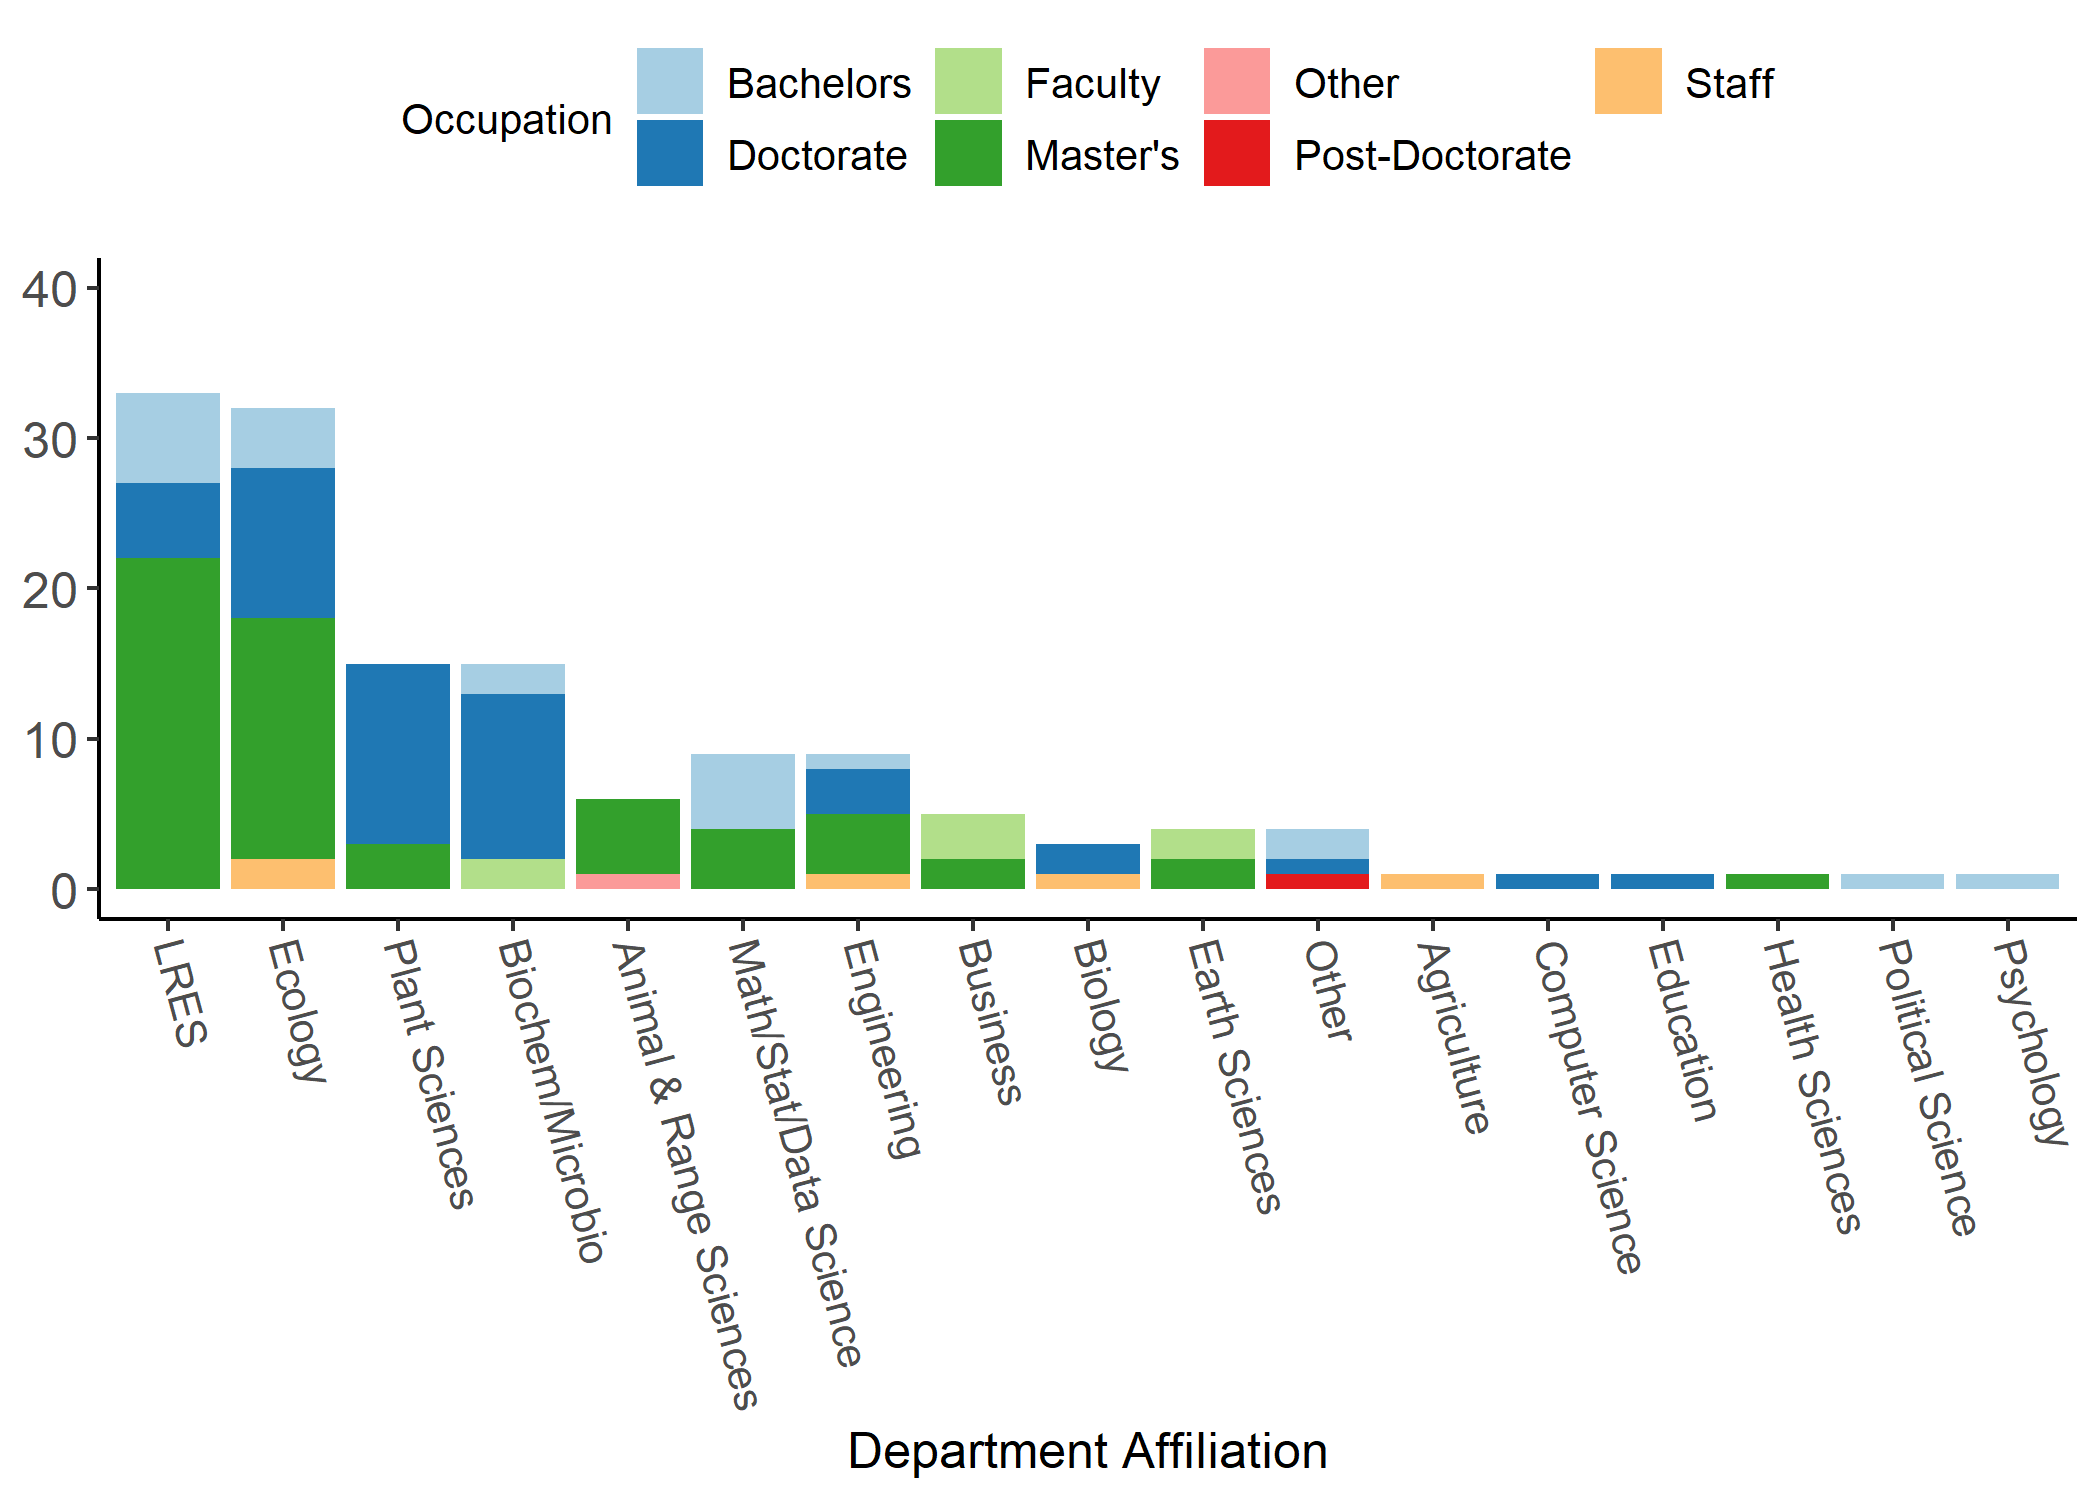
\includegraphics[width = \textwidth]{images/better_colors_attendance.png}
\caption{Number of attendees by department and current occupation, selected from
an itemized list of campus departments and positions.}
    \label{fig:departments}
\end{figure}
}

\quad Consistent with the environmental science literature \citep{andelman, 
hampton, hernandez, datacarpentry}, a large number of workshop participants were
either unfamiliar with the concept of a programming language or had no
experience with any programming languages. Nearly 60\% of attendees reported no
experiences with any programming languages, 20\% reported experiences working in
\texttt{R}, and 30\% reported experiences with other programming languages (e.g.
MatLab, SQL, Java, C). 

\quad Many attendees, however, stated that they had taken courses in statistics.
The majority of participants reported having either undergraduate or graduate
experiences with an introductory level statistics course. Notably, over 15\% of
attendees reported having no formal statistical training. Most graduate students
had enrolled in discipline-specific introductory statistics courses in their own
department or a graduate-level applied statistics course offered by the
Department of Mathematical Sciences. Table \ref{tab:statistics} consolidates 
themes of workshop participants' previous statistical experiences, when asked to
report the statistics courses they have taken over the course of their
education. 

{\spacingset{1.05}
\begin{table}[h!]
    \centering
    \begin{tabular}{lc}
\hline
Stat Courses & Participants \\
\hline
Introductory Statistics & 46 \\
Applied Statistics & 42 \\
None & 24 \\
Discipline Specific Introductory Statistics & 20 \\
Intermediate Statistics & 10 \\
Experimental Design	& 8 \\
Probability Theory	& 6 \\
Statistical Computing & 3 \\
Sampling & 3 \\
Biostatistics & 2 \\
Spatial Analysis & 2 \\
Econometrics & 1 \\
Time Series Analysis & 1 \\
\hline
\end{tabular}
\caption{Workshop attendees' responses to the question ``What are your previous
statistical experience(s)?  List course names.,'' thematically organized based
on content of the course.}
\label{tab:statistics}
\end{table}
}

\subsection{Motivation for Attending} 

\quad As expected from the prevalence of the use of \texttt{R} in environmental
science research \citep{Rpopular, mislan}, over half of the master's, doctoral, 
and post-doc workshop participants attended for assistance with their research. 
Others were seeking additional assistance for learning the \texttt{R} skills
necessary for their coursework, refreshing or updating their \texttt{R}
skills to include new tools they were unfamiliar with(e.g. \texttt{ggplot}, 
\texttt{dplyr}), or undergraduates preparing for graduate school.  

\quad As echoed by previous studies of environmental science graduate students
\citep{datacarpentry, theobold}, attendees overwhelmingly stated that they
primarily use the internet (27\%), their peers (21\%), or their lab mates (15\%) 
when learning \texttt{R}. Based on the statistical backgrounds of these
participants and the statistics education literature on computing in the
statistics classroom, it is not surprising that nearly two-thirds of these 
individuals reported using resources other than course materials as their main 
resource for learning \texttt{R}. 

\subsection{Reflections of Workshop Participants} 

\quad The percentage of individuals reporting that all of the information
presented was new to them differed by workshop, with 40\% of \emph{Introduction
to \texttt{R}} participants, 30\% of \emph{Intermediate \texttt{R}}
participants, 80\% of \emph{Data Wrangling} participants, and 50\% of 
\emph{Data Visualization} participants stating the information was new to them.
Across every workshop, nearly all participants stated that they ``strongly
agreed'' that they ``learned skills that [they] will be able to use in [their]
research/work.'' Over 75\% of the workshop participants reported that they would
use the skills they learned in their research immediately or in the next 30
days. 

\quad The themes which emerged from these attendees' reflections to what they 
enjoyed most about the workshop were hands-on learning, workshop atmosphere,
instructor attributes, and confidence. Many attendees felt walking through the
code step-by-step and the hands-on exercises ``fostering a much greater level of
understanding'' and left them feeling more ``confident figuring things out on my
own.'' Furthermore, these attendees voiced that the workshop left them feeling
more independent, because ``I have a better understanding of how to read code, 
what certain symbols/terms/etc mean and how they work.'' Individuals who
reported using the internet as a resource to learn \texttt{R} stated that
``it's easy to walk away from \texttt{R} workshops wondering if anything was
learned, however the exercises were a clear tool which allow me to see what I 
gained.''  

\section{Sustainability of Workshops}  
\label{sec:sustainability}

\quad To facilitate the sustainability of these workshops, we forged a
partnership between our institution's library and the Department of Mathematical
Science's Statistical Consulting and Research Services (SCRS). We believe a 
university's library is an optimal unit for offering these workshops, as it is
both department-agnostic and a central hub for the entire university community.
Furthermore, by partnering with a organization that provides statistical
consulting, workshop participants are provided with a potential avenue if
difficulties or additional questions arise---so the peer network is not shifted 
onto workshop instructors. 

\quad A data-engagement grant from the National Network of Libraries of Medicine
during the 2018-2019 academic year supported the primary author in leading the
workshops, becoming a Carpentries certified instructor, and incorporating the
results of this research into the broader Data and Software Carpentry curricula.
A \$5,000 faculty excellence grant during the 2019-2020 academic year,
facilitated the implementation of a ``train-the-trainer'' model, training two 
future graduate student instructors. Students were recruited from the masters
and doctoral programs in statistics, but because of the widespread use of 
\texttt{R} across scientific fields, students from a variety of backgrounds hold
the potential to be effective instructors. Both semesters, the authors met with 
these students for one hour a week to build students' facilities and confidence
instructing each workshop. Each of these semesters, students taught different 
30 to 45 minute portions of each workshop during, and acted as assistants for
the remainder for the workshop.  

% \quad Currently, this design research is focusing on incorporating the content of these workshops into the \emph{Data Analysis and Visualization in \texttt{R}} lesson within Data Carpentry's Ecology curriculum. Infusing the skills outlined in this research into the \emph{Data Analysis and Visualization in \texttt{R} for Ecologists} lesson helps to create a Carpentries curriculum that best reflects the ``core data skills'' necessary for data-intensive environmental science research. For skills outlined by this research where there is no room in the current \emph{Data Analysis and Visualization in \texttt{R} for Ecologists} lesson, the Carpentries Incubator and Carpentries Lab provide potential avenues to produce additional lesson materials that are broadly available to The Carpentries community. These avenues allow for the continued discussion of the importance of integrating user-defined functions, conditional statements, and loops into the broader Data Carpentry Ecology curriculum.    

\quad The Carpentries does not require training for instructors to use their
content, as The Carpentries materials are publicly available for use and 
adaptation (with acknowledgement). However, if the instructor or institution
desires to advertise their workshops as Carpentries workshops there are two 
options: (1) the lead instructor is a Carpentries certified instructor, or (2)
the institution requests a workshop through The Carpentries, who then recruits 
instructors for a fee. Through the primary author completing The Carpentries
instructor training, we were able to offer self-organized workshops interweaving 
the content from both Data and Software Carpentry workshops. Additionally, 
through this experience the primary author was able to guide the future 
workshop instructors through the process of becoming Carpentries certified
instructors. 

\quad Similar to the Explorations in Statistics Research workshop model 
\citep{esr}, the ``standard'' Carpentries workshop format takes place over an 
intensive two days. Self-organized workshops allow for the added flexibility of 
tailoring this format to be more conducive for busy students, faculty, and
staff. This revised format has both benefits and costs. The additional time
between each workshop helps to alleviate the brain fatigue often experienced in
intensive workshops, and allows for participants to attend the workshops that 
are relevant to the skills they wish to acquire. However, in this extended
format, workshops after \emph{Introduction to \texttt{R}} are potentially
considered ``specialized'' workshops and experience lower attendance. At an
academic institution, there is the possibility of integrating this type of 
workshop series into a single credit course. When considering this as an option, 
however, institutions should think critically about how faculty and staff can 
still participate in these critical learning opportunities. Alternatively,
institutions could offer undergraduate students the option of assisting in the 
implementation of these workshops for course credit, and allow for the
possibility of students becoming lead or co-instructors as they progress through
their program. 

\section{Limitations \& Future Research} 
\label{sec:future}

\quad The sentiments heard by faculty members in this research, unearth the
possibility that many faculty may be unaware of the computing skills necessary
for their graduate students to participate in the entire data analysis cycle.
Instead, students may have more relevant knowledge regarding the data science
skills that are necessary for their research. Hence, the next iteration of this
design work will be informed by the collection of the research (\texttt{R}) code
produced by environmental science graduate students. Graduate students' research
code acts as artifacts of their research experience, providing ``mute evidence''
\citep{hodder} of the data science skills necessary throughout the data analysis
cycle. The skills outlined by this research aid in reevaluating the content of
these workshops, to ensure they cover the skills necessary for graduate-level
environmental science research. 

\quad Additionally, the attendance of these tailored workshops by students,
faculty, and staff from disciplines outside of the environmental sciences brings
to question whether this type of tailored design work is necessary. Over a third
of the workshop attendees came from disciplines outside of the environmental 
sciences, and, strikingly, these attendees reported similar workshop experiences
to attendees from these targeted disciplines. This brings to question if there
are common computational understandings necessary for research in \emph{any}
scientific field, which should be infused into \emph{every} statistics and data
science course. Alternatively, we saw a greater persistence across workshops by 
attendees from environmental science fields. This made us wonder, what are the
drivers behind these individuals' continued attendance? Future research 
investigating the learning outcomes of workshop attendees holds the potential to 
provide fruitful insight on the necessity of discipline-specific learning
opportunities. 

% Research on drift/questions in WS
\quad Finally, despite the increasing availability of extracurricular 
workshops, research has yet to investigate the consistency or drift of these 
workshops. In this research, because of the large attendance at many
\emph{Introduction to \texttt{R}} workshops, a large number of questions would
arise over the course of the afternoon. This lead to an inability to cover some
of the workshop content in as much depth as hoped, yet some attendees remarked 
that ``with so many people, [the workshop] had better discussions.'' A large 
scale analysis of the content covered by these workshops could unearth common
questions or misunderstandings, aiding in the reconstruction of lessons to
better scaffold learning. 

\section{Conclusion}
\label{sec:conclusion}

\quad Ten years ago, Nolan and Temple Lang declared that ``modernizing the
statistics curricula to include computing [...] is an issue that deserves
widespread attention and action'' (p.\ 106). Over the last ten years, we have
seen both small \citep{gaise} and large \citep{asa} changes advocated to the
statistics curriculum. Unfortunately, changes to graduate-level statistics
service courses has received less attention and poses different issues. 

\quad Statistics courses that serve a variety of students (undergraduate,
graduate, statistics major, non-major) reflect a snapshot of the statistics
curriculum, but often act as many students' sole statistics course prior to
conducting scientific research. Instructors of these courses thus grapple with 
difficult decisions of how they can ensure their students have both the
statistical and ``computational understanding, skills, and confidence needed to
actively and wholeheartedly participate'' in the scientific research arena 
\citep[p.\ 106]{nolan}. For instructors unfamiliar with students' scientific
disciplines, it can be difficult to ``be bold and design curricula from
scratch'' \citep[p.\ 106]{nolan}. The topics suggested by Nolan and Temple Lang
(2010) represent a starting point toward building a taxonomy for computing in
statistics for undergraduate and graduate statistics programs. These topics,
however, may not be relevant to or emphasized by other scientific disciplines
whose students enroll in graduate-level statistics service courses.  In our
research, we found that environmental science faculty stressed the importance of
graduate students developing skills surrounding the fundamentals of working with
data in \texttt{R}, software skills for data processing and preparation, 
creation of data visualizations, and usage of reproducible work flows. 

\quad The time is ripe for us to ``update the foundational concepts and
infrastructure'' \citep[p.\ 5]{crossroads} included in statistics service
courses, in the new era of data science. As we work toward a more thorough
integration of computing into these courses, this research offers a model for
facilitating external workshops, which hold the potential to fill a critical
hole in the curriculum of many college programs. External workshops hold the
opportunity for co-curricular learning, when paired with statistics service
courses, so students leave their statistics service course with the computing
skills necessary to engage in the entire data analysis cycle. Moreover, these
workshops support university-wide data science literacy, facilitating avenues
for faculty to acquire data science knowledge and skills which ``they have not
had the opportunity to learn well'' \citep[p.\ 106]{nolan}, and providing
resources for instructors to meaningfully integrate discipline-specific
computing skills into their classroom. 

% Additionally, because workshops are able to thrive outside of university
% curricula, they hold the ability to ``adapt materials rapidly and remain on the
% leading edge of technological development'' \citep[p.\ 547]{hampton}.
% Furthermore, workshops offer the opportunity for a wide variety of researchers,
% not just students, to acquire the data science skills necessary for
% data-intensive research, supporting the broader community of researchers. 

% This collaboration 
% is critical when developing resources for researchers in the broader scientific
% community, as the discipline of Statistics was developed to support research in
% other scientific disciplines to evaluate evidence obtained from data. 

\section{Acknowledgements}

We would like to specially thank the participants from this study, without whom
this research would not have been possible. We would also like to thank the 
workshop helpers for their time and assistance, helping to grow the data 
literacy across our campus. Lastly, we thank Mary Alice Carlson, Jennifer Green,
Mark Greenwood, Megan Wickstrom, editor Johanna Hardin, and the reviewers for
their insightful comments on this paper. 

\bibliography{ref}
\bibliographystyle{apalike}

\end{document}
